\documentclass[../main.tex]{subfiles}

\usepackage{float} % Librería para presentación de imágenes

\begin{document}

La página Web va a permitir a los usuarios acceder de forma concisa a la información que queremos presentar. Se van a hacer dos interfaces, una para investigadores y otra para usuarios que simplemente quieran informarse. Se va añadir una interfaz que se muestre al inicio de la aplicación donde los usuarios elijan que interfaz desean ver.

\subsection{Interfaz inicio}

Esta interfaz va a constar de dos botones, uno que redirija a la interfaz de usuarios y otro a la de investigadores, como se puede comprobar en la imagen \ref{inc}.

\begin{figure}[ht]
    \centering
    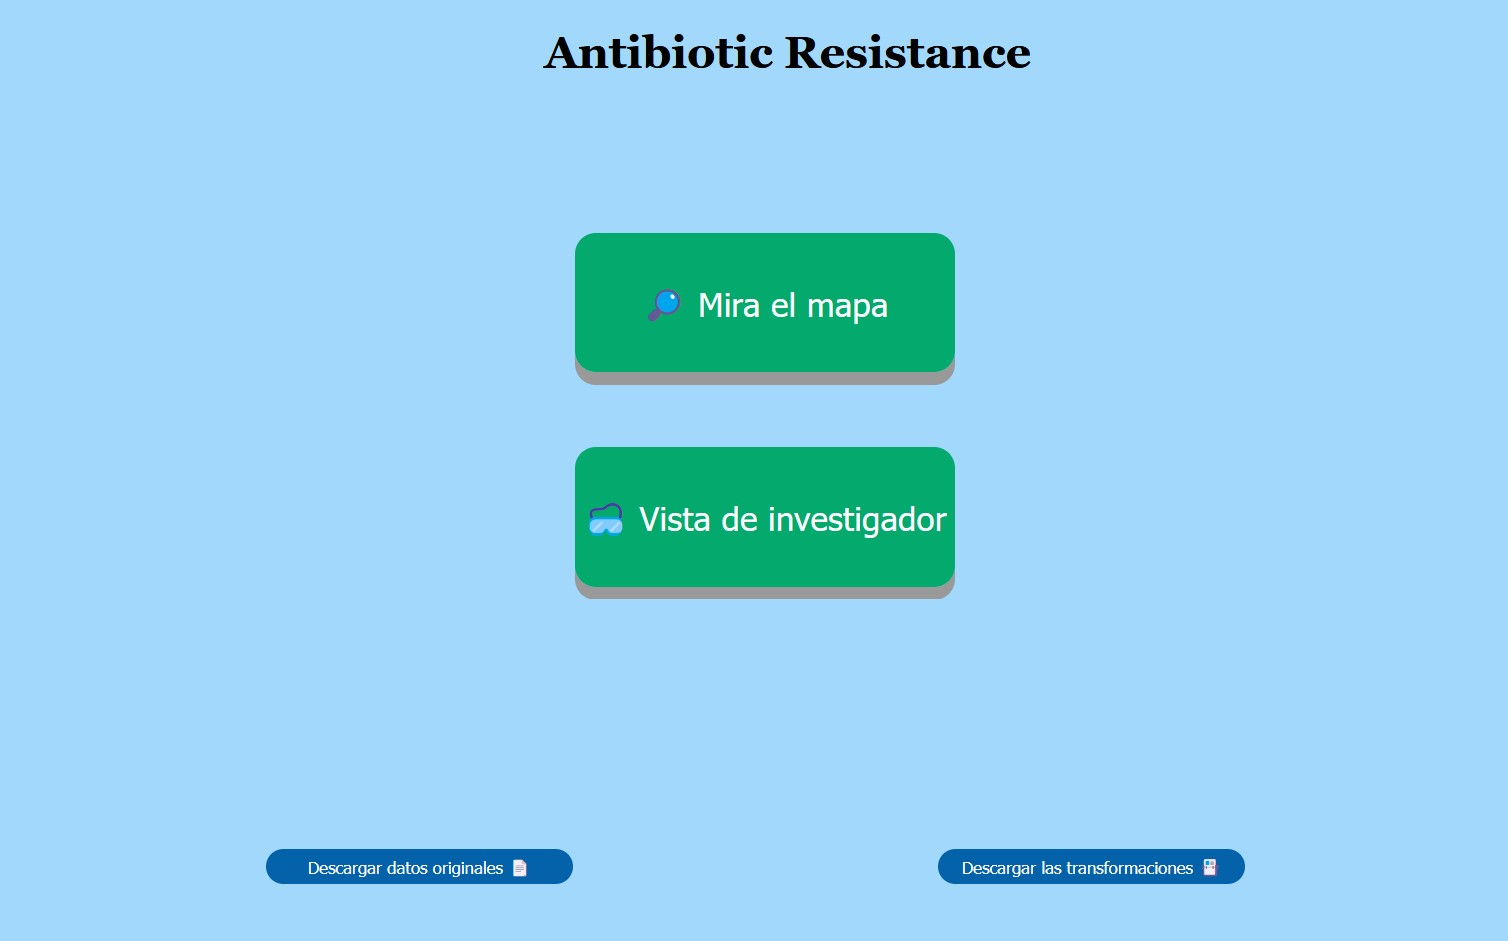
\includegraphics[scale=0.65]{inicio}
    \caption{Interfaz Inicio}
    \label{inc}
\end{figure}

\subsection{Interfaz investigadores}

Esta interfaz esta enfocada para personas dedicadas a la investigación. A la izquierda de la interfaz van a encontrarse dos botones y a la derecha una tabla. Al seleccionar uno de los botones de la izquierda (el de la imagen de una bacteria), en la tabla de la derecha se presentará información relacionada con las bacterias, los antibióticos a los que son resistentes y el porcentaje de resistencia de la bacteria en ese estudio (es decir, se filtran de las columnas del dataset aquellas columnas de interés). Esto se refleja en la imagen \ref{invBac}.

\begin{figure}[ht]
    \centering
    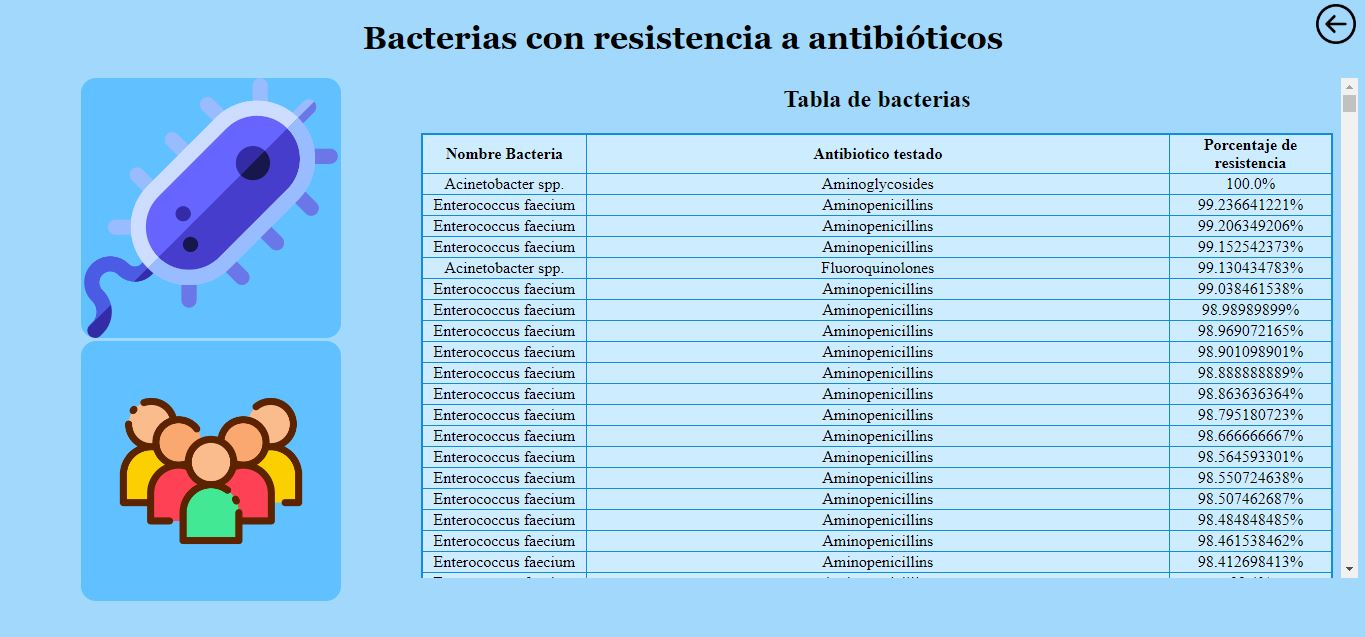
\includegraphics[scale=0.4]{images/investigador_bacteria.JPG}
    \caption{Tabla bacterias}
    \label{invBac}
\end{figure}


En el caso de seleccionar el otro botón en la tabla de la derecha se presentará la información relacionada con los grupos a los que se le realizó el estudio (imagen  \ref{invEst}).

\begin{figure}[ht]
    \centering
    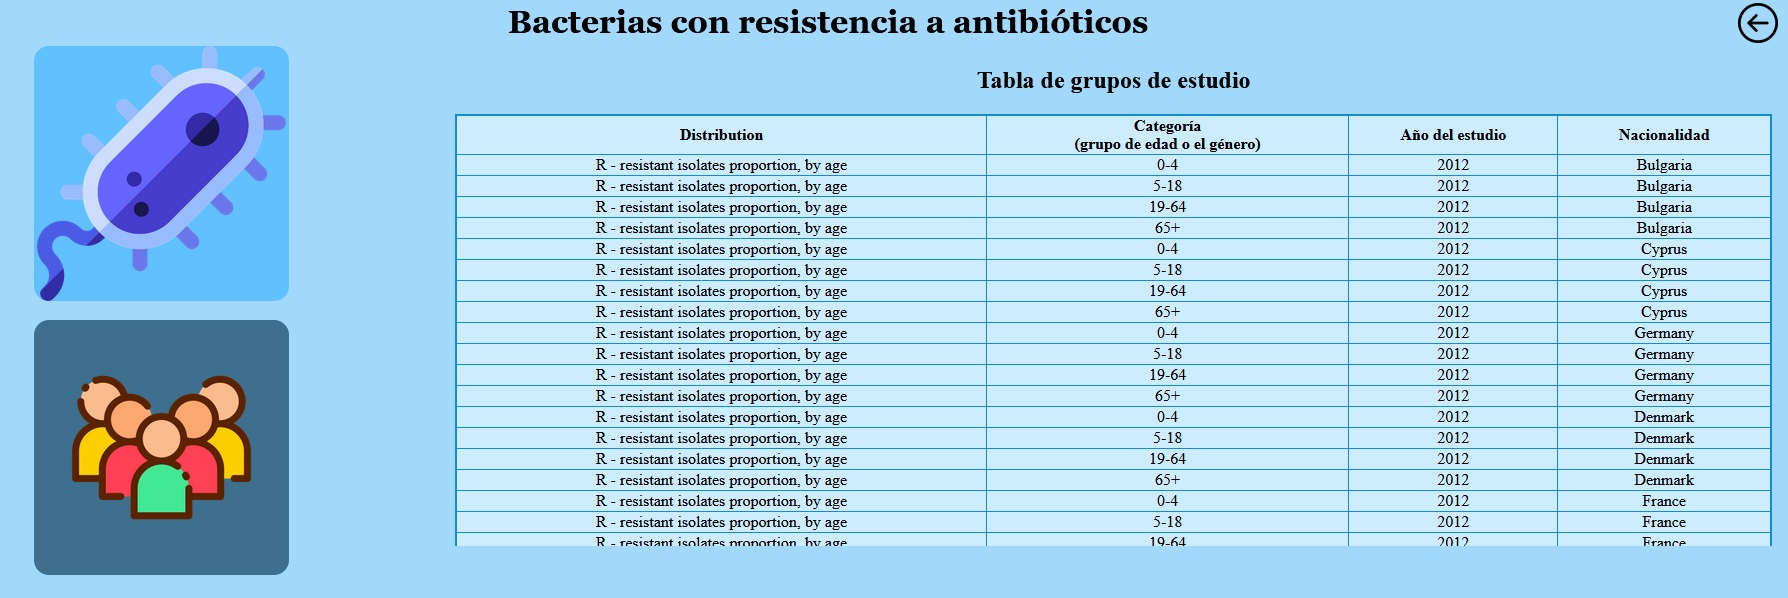
\includegraphics[scale=0.4]{images/investigador_estudio.JPG}
    \caption{Tabla estudios}
    \label{invEst}
\end{figure}

\subsection{Interfaz usuarios}

En este interfaz se presenta un mapa de Europa. Delante de este mapa se van a poner una serie de botones por zonas (que incluyan más de un país) para que el usuario pueda hacer click y obtener información sobre aquellas bacterias con resistencia a antibióticos en esa zona de Europa.

\end{document}